\documentclass[a4paper,11pt,dvipdfmx]{ujarticle}
% パッケージ
\usepackage{graphicx}
\usepackage{url}
% レイアウト指定を記述したファイルの読み込み
\input{layout}

% タイトルと氏名を変更せよ．
\title{日本におけるデジタル化の状況}
\author{G684532026 小林 遼大}

\begin{document}

\maketitle %ここにタイトルが入る

% ここから本文
\section{ブロードバンドの整備状況}
OECDによるブロードバンド回線の普及に関する調査\cite{oecd}によると, 図\ref{fig:fig21}に示すように, 日本における100人あたりのモバイルブロードバンドの加入者数は190.5で, 第1位になっている. 2位はエストニアで, 3位は米国と続く.

% 本文(1)
%  参考文献の参照: \cite{}
%  図番号の参照： \ref{}
% を使う
% 文献データベースのキーワードは oecd と imd
% になっている．

\begin{figure}[htbp]
    \centering
    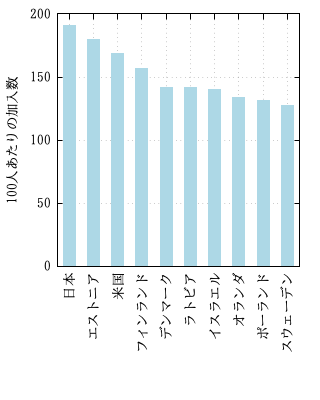
\includegraphics{fig21.png}
    \caption{光ファイバー回線の加入者数}\label{fig:fig21}
\end{figure}
% \begin{figure}[htbp]
% \end{figure}
% で囲み
% \caption{}
% で図のタイトルを入れる．
% \label{}
% を使って図番号が参照できるようにする
% また，
% \centering
% で図が中央に来るようにする

% ーーー
\section{デジタル競争力ランキング}
国際経営開発研究所(IMD)の調査\cite{imd}によると, 表\ref{tbl:mytbl}に示すように, 日本のデジタル競争力ランキングは調査対象の64カ国中, 総合で28位, 知識分析で25位となっている.
% 本文(2)

\begin{table}[htbp]
    \centering
    \caption{デジタル競争力ランキング(64か国中)}\label{tbl:mytbl}
    \begin{tabular}{|c|c|c|}
    \hline
    国 & 総合 & 知識 \\ 
    \hline
    米国 & 1位 & 3位 \\
    \hline
    香港 & 2位 & 5位 \\
    \hline
    スウェーデン & 3位 & 2位 \\
    \hline
    デンマーク & 4位 & 8位 \\
    \hline
    シンガポール & 5位 & 4位 \\
    \hline
    \hline    
    韓国 & 12位 & 15位 \\
    \hline
    中国 & 15位 & 6位 \\
    \hline
    \hline    
    日本 & 28位 & 25位 \\
    \hline
    \end{tabular}  
\end{table}     
% による表の記述を 
% \begin{table}[htbp]
% \end{table}
% で囲み
% \caption{}
% で表のタイトルを入れる．
% \label{}
% を使って表番号が参照できるようにする
% また，
% \centering
% で表が中央に来るようにする

% ーーー
\section{考察}
\begin{itemize}
    \item 日本はブロードバンド回線の普及率が非常に高く世界一位であるが, デジタル競争力では低い水準にとどまっていることから, 国全体として回線の発展が進めるだけではデジタル技術の発展や活用に繋がっていないことが考えられる. 
    \item 米国はどちらの指標でも上位に位置していることから, 回線の普及だけでなく, デジタル技術の発展にも力を入れていることが考えられる.
\end{itemize}
% 考察
%
% \begin{itemize}
% \end{itemize}
% を使って箇条書きで記述する

% ここに参考文献が入る
\bibliographystyle{junsrt}
\cite{oecd,imd}
\bibliography{exercise.bib}

\end{document}